\documentclass{standalone}

\usepackage{tikz}
\usetikzlibrary{arrows}
\usetikzlibrary{decorations.markings}
\usepackage{standalone}

\begin{document}

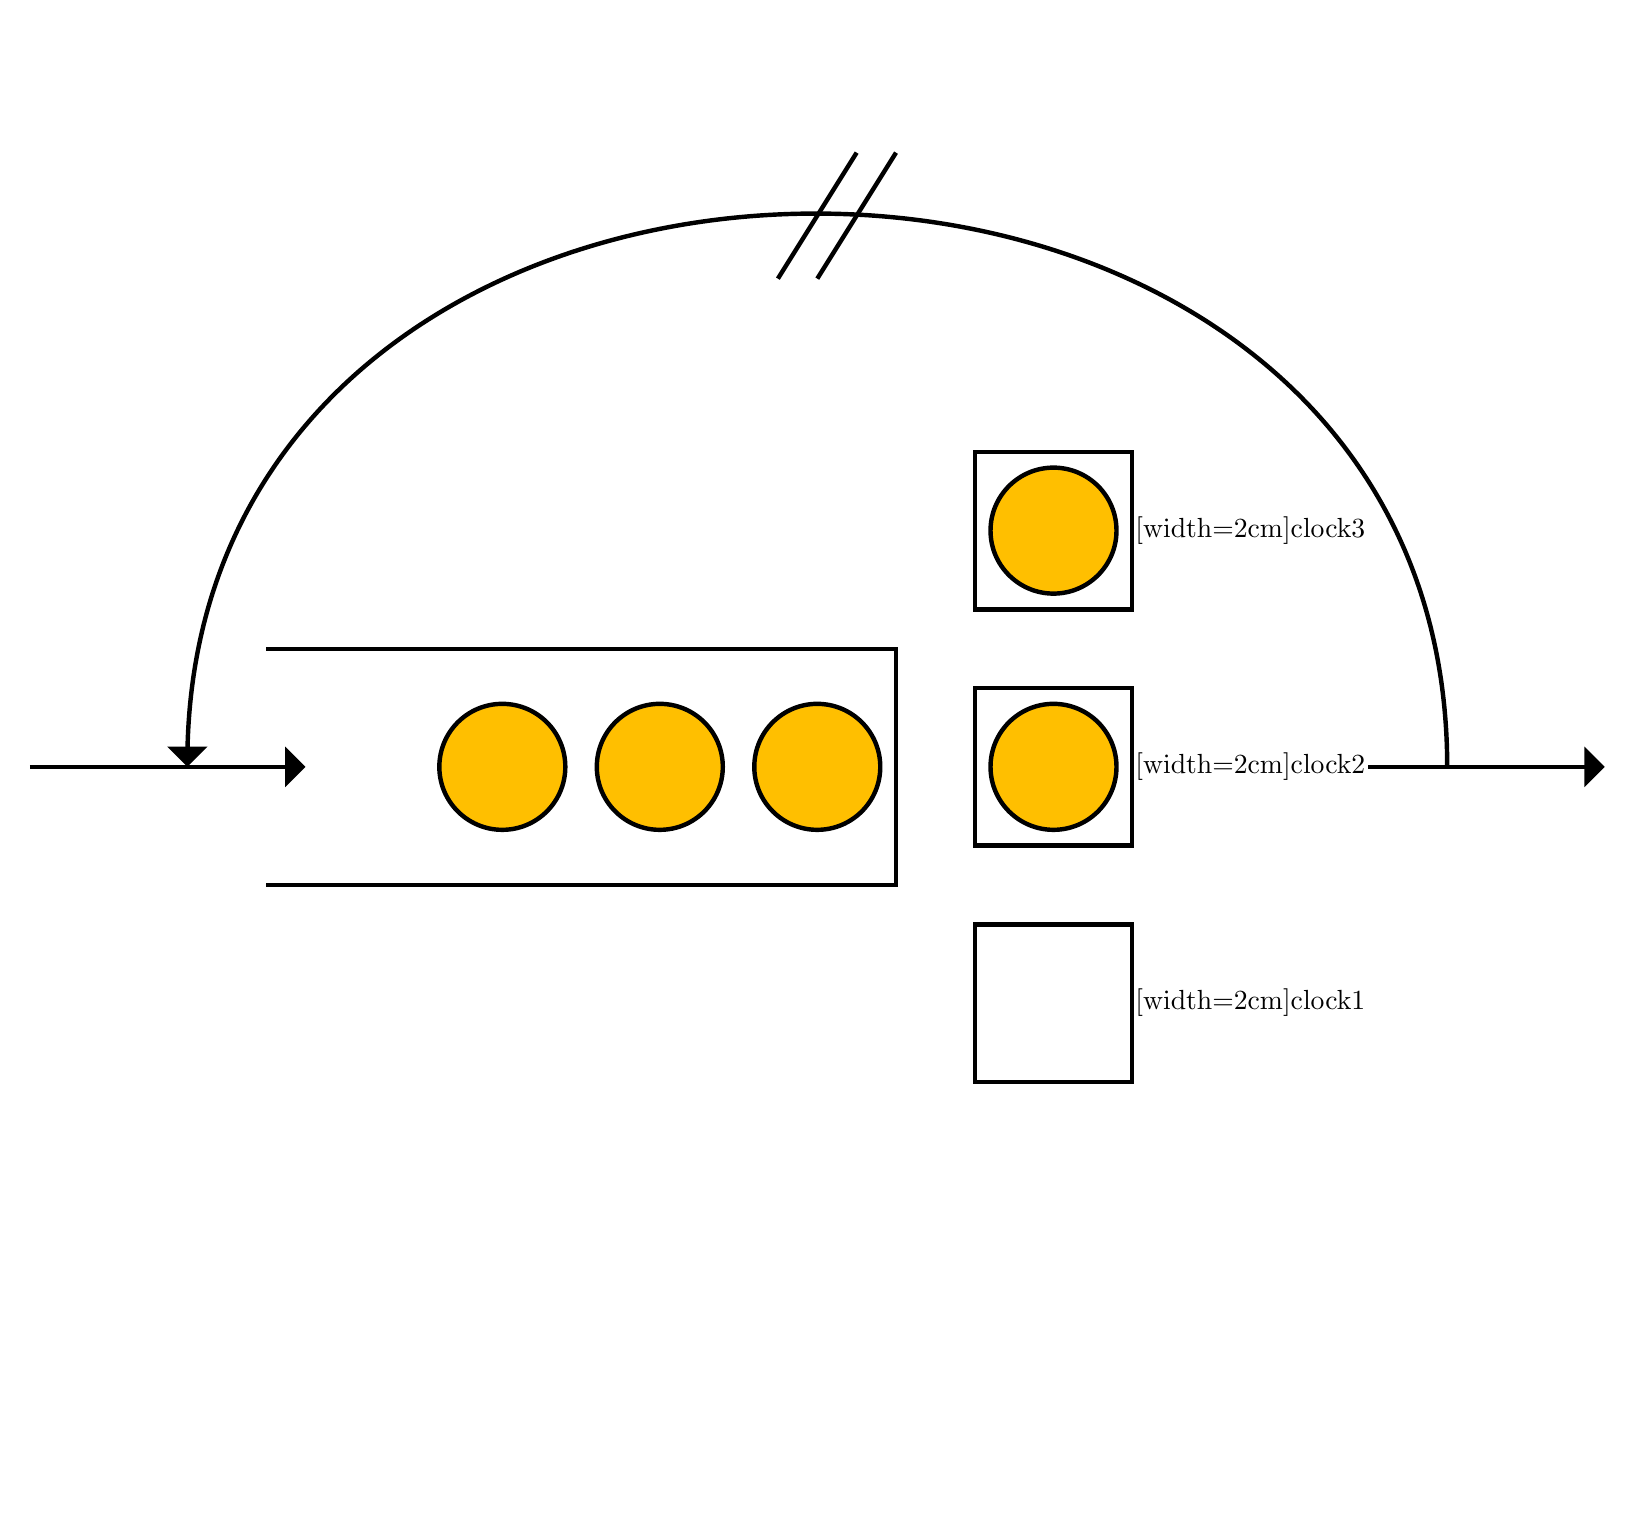
\begin{tikzpicture}


\draw[ultra thick] (-9,2.5) -- (-1,2.5) -- (-1,5.5) -- (-9,5.5);

\draw[ultra thick] (0, 0) rectangle (2, 2);
\draw[ultra thick] (0, 3) rectangle (2, 5);
\draw[ultra thick] (0, 6) rectangle (2, 8);
\node at (3.5, 1) {\includestandalone[width=2cm]{clock1}};
\node at (3.5, 4) {\includestandalone[width=2cm]{clock2}};
\node at (3.5, 7) {\includestandalone[width=2cm]{clock3}};

\draw[ultra thick, -triangle 90] (-12, 4) -- (-8.5, 4);
\draw[ultra thick, -triangle 90] (5, 4) -- (8, 4);
\draw (6, 4) edge[ultra thick,-triangle 90,out=90,in=90,looseness=1.5] (-10,4);
\draw (6, 4) edge[ultra thick,-triangle 90,out=-90,in=-90,looseness=1.5,draw=none] (-10,4);

\draw[ultra thick] (-2.5,10.2) -- (-1.5,11.8);
\draw[ultra thick] (-2,10.2) -- (-1,11.8);

\draw[ultra thick, draw=black,fill=orange!50!yellow] (1,7) circle (0.8);
\draw[ultra thick, draw=black,fill=orange!50!yellow] (1,4) circle (0.8);
\draw[ultra thick, draw=black,fill=orange!50!yellow] (-2,4) circle (0.8);
\draw[ultra thick, draw=black,fill=orange!50!yellow] (-4,4) circle (0.8);
\draw[ultra thick, draw=black,fill=orange!50!yellow] (-6,4) circle (0.8);

\end{tikzpicture}

\end{document}
